% Options for packages loaded elsewhere
\PassOptionsToPackage{unicode}{hyperref}
\PassOptionsToPackage{hyphens}{url}
%
\documentclass[
  11pt,
]{article}
\usepackage{amsmath,amssymb}
\usepackage{lmodern}
\usepackage{iftex}
\ifPDFTeX
  \usepackage[T1]{fontenc}
  \usepackage[utf8]{inputenc}
  \usepackage{textcomp} % provide euro and other symbols
\else % if luatex or xetex
  \usepackage{unicode-math}
  \defaultfontfeatures{Scale=MatchLowercase}
  \defaultfontfeatures[\rmfamily]{Ligatures=TeX,Scale=1}
\fi
% Use upquote if available, for straight quotes in verbatim environments
\IfFileExists{upquote.sty}{\usepackage{upquote}}{}
\IfFileExists{microtype.sty}{% use microtype if available
  \usepackage[]{microtype}
  \UseMicrotypeSet[protrusion]{basicmath} % disable protrusion for tt fonts
}{}
\makeatletter
\@ifundefined{KOMAClassName}{% if non-KOMA class
  \IfFileExists{parskip.sty}{%
    \usepackage{parskip}
  }{% else
    \setlength{\parindent}{0pt}
    \setlength{\parskip}{6pt plus 2pt minus 1pt}}
}{% if KOMA class
  \KOMAoptions{parskip=half}}
\makeatother
\usepackage{xcolor}
\usepackage[margin=1.0in]{geometry}
\usepackage{graphicx}
\makeatletter
\def\maxwidth{\ifdim\Gin@nat@width>\linewidth\linewidth\else\Gin@nat@width\fi}
\def\maxheight{\ifdim\Gin@nat@height>\textheight\textheight\else\Gin@nat@height\fi}
\makeatother
% Scale images if necessary, so that they will not overflow the page
% margins by default, and it is still possible to overwrite the defaults
% using explicit options in \includegraphics[width, height, ...]{}
\setkeys{Gin}{width=\maxwidth,height=\maxheight,keepaspectratio}
% Set default figure placement to htbp
\makeatletter
\def\fps@figure{htbp}
\makeatother
\setlength{\emergencystretch}{3em} % prevent overfull lines
\providecommand{\tightlist}{%
  \setlength{\itemsep}{0pt}\setlength{\parskip}{0pt}}
\setcounter{secnumdepth}{5}
\newlength{\cslhangindent}
\setlength{\cslhangindent}{1.5em}
\newlength{\csllabelwidth}
\setlength{\csllabelwidth}{3em}
\newlength{\cslentryspacingunit} % times entry-spacing
\setlength{\cslentryspacingunit}{\parskip}
\newenvironment{CSLReferences}[2] % #1 hanging-ident, #2 entry spacing
 {% don't indent paragraphs
  \setlength{\parindent}{0pt}
  % turn on hanging indent if param 1 is 1
  \ifodd #1
  \let\oldpar\par
  \def\par{\hangindent=\cslhangindent\oldpar}
  \fi
  % set entry spacing
  \setlength{\parskip}{#2\cslentryspacingunit}
 }%
 {}
\usepackage{calc}
\newcommand{\CSLBlock}[1]{#1\hfill\break}
\newcommand{\CSLLeftMargin}[1]{\parbox[t]{\csllabelwidth}{#1}}
\newcommand{\CSLRightInline}[1]{\parbox[t]{\linewidth - \csllabelwidth}{#1}\break}
\newcommand{\CSLIndent}[1]{\hspace{\cslhangindent}#1}
\newcommand{\bcenter}{\begin{center}}
\newcommand{\ecenter}{\end{center}}
\newcommand{\btitlepage}{\begin{titlepage}}
\newcommand{\etitlepage}{\end{titlepage}}
\usepackage{setspace}\doublespacing
\usepackage{helvet}
\renewcommand*\familydefault{\sfdefault}
\usepackage{booktabs}
\usepackage[font=small,labelfont=bf]{caption}
\usepackage{booktabs}
\usepackage{longtable}
\usepackage{array}
\usepackage{multirow}
\usepackage{wrapfig}
\usepackage{float}
\usepackage{colortbl}
\usepackage{pdflscape}
\usepackage{tabu}
\usepackage{threeparttable}
\usepackage{threeparttablex}
\usepackage[normalem]{ulem}
\usepackage{makecell}
\usepackage{xcolor}
\ifLuaTeX
  \usepackage{selnolig}  % disable illegal ligatures
\fi
\IfFileExists{bookmark.sty}{\usepackage{bookmark}}{\usepackage{hyperref}}
\IfFileExists{xurl.sty}{\usepackage{xurl}}{} % add URL line breaks if available
\urlstyle{same} % disable monospaced font for URLs
\hypersetup{
  hidelinks,
  pdfcreator={LaTeX via pandoc}}

\author{}
\date{\vspace{-2.5em}}

\begin{document}

\begin{titlepage}

\begin{center}

\vspace*{30mm}

\hypertarget{this-is-an-awesome-title}{%
\section*{\texorpdfstring{\textbf{This is an awesome
title}}{This is an awesome title}}\label{this-is-an-awesome-title}}
\addcontentsline{toc}{section}{\textbf{This is an awesome title}}

\vspace{30mm}

Yurun Ying\textsuperscript{1}, Pekka
Santtila\textsuperscript{1,2,\(\dagger\)}

\textsuperscript{1} Faculty of Arts and Sciences, NYU Shanghai

\textsuperscript{2} NYU-ECNU Institute for Social Development at NYU
Shanghai

\end{center}

\vspace{40mm}

\textsuperscript{\(\dagger\)} To whom correspondence should be
addressed:

\end{titlepage}

\newpage

\hypertarget{abstract}{%
\section*{Abstract}\label{abstract}}
\addcontentsline{toc}{section}{Abstract}

Gender differences in short-term mating behaviors have been a
well-documented phenomenon in human sexuality research. Existing studies
usually conflate gender differences in preferences for short-term mating
with differences in sexual behaviors, which is theoretically dubious.
Using an agent-based model, the present study investigated whether men
and women's different mating preferences resulted in any gender
differences in short-term mating behaviors, and if they did, under what
circumstances. The results suggested that heterosexual men and women had
the same average number of short-term mating experiences and short-term
mates even when gender differences in preferences fort-term mating
existed. Gender differences in mating behaviors only emerged when
heterosexual men and women in the mating pool were considered. Moreover,
gay men had a higher average number of both outcomes than lesbian women
and than heterosexual men under such a circumstance. These results
suggest that theoretically speaking, gender differences in short-term
mating behaviors only occurred among particular populations, or when
men's preferences for short-term mating are not constrained by those of
women. Suggestions for future research in human mating psychology and
behaviors were provided.

~

\emph{Keywords:} agent-based modeling, short-term mating, casual sex,
sexual strategy theory, female choice hypothesis

\newpage

\hypertarget{introduction}{%
\section{Introduction}\label{introduction}}

Gender differences in sexual behaviors, especially short-term mating
behaviors, have been a well-documented phenomenon in human sexuality
research. For example, research has found that heterosexual men, as
compared to heterosexual women, have a higher average number of past
short-term sexual partners (Oliver \& Hyde, 1993; Petersen \& Hyde,
2010; Rissel et al., 2014), have short-term mating more frequently
(Petersen \& Hyde, 2010), and engage in extramarital sex more often
(Petersen \& Hyde, 2010). These gender differences have also been
observed between gay men and lesbian women (Bailey et al., 1994; Bryant
\& Demian, 1994; Peplau et al., 1997, 2004).

In the existing literature, gender differences in sexual behaviors are
not usually distinguished from those in attitudes towards or preferences
for short-term mating. Some researchers study gender differences on the
two levels simultaneously without a conceptual distinction (e.g.,
Petersen \& Hyde, 2010), whereas some implicitly equate the two,
assuming that behavioral differences are a direct expression of the
psychological ones (e.g., Schmitt et al., 2001).

Intuitive as this line of reasoning is, there are good reasons to doubt
its soundness. This is because any heterosexual sexual encounter
involves both a man and a woman (the frequency of encounters involving
more than two persons is negligible, (e.g., Herbenick et al., 2017). A
new short-term mating experience for a man is, therefore, also a new
experience for a woman, and the same logic applies to counting a new
short-term mate. As a result, the psychological differences in
short-term mating preferences may not result in behavioral ones in the
heterosexual case (Archer, 2019).

The present study took gender differences in mating preferences as an
assumption, which was proposed by sexual strategy theory (Buss \&
Schmitt, 1993) and repeatedly found support by empirical studies (e.g.,
Schmitt, 2003; Walter et al., 2020). Using an agent-based model, we
investigated whether men and women's different mating preferences
resulted in any gender differences in short-term mating behaviors,
specifically, in the number of short-term mating experiences and
short-term mates, and if they did, under what circumstances.

\hypertarget{gender-differences-in-short-term-mating-preferences}{%
\subsection{Gender differences in short-term mating
preferences}\label{gender-differences-in-short-term-mating-preferences}}

Gender differences in mating strategies have been studied in the light
of sexual strategy theory (Buss \& Schmitt, 1993). It posits that since
the minimum investment that men devote to their offspring (contribution
of sperm through one sexual act) is lower than that of women (gestation,
labor, and lactation), men tend to have short-term mating as a larger
part of their mating strategy than women do. This is because women's
high minimum investment leads to higher opportunity cost (vs.~men) if
they have sex with a suboptimal partner and give birth to offspring with
a low survival chance. As a result, men may have a greater interest in
short-term mating, desire a larger number of short-term mates in a given
period, and be less selective with respect to accepting a potential mate
(Buss \& Schmitt, 1993).

The hypotheses derived from sexual strategy theory have received
extensive support from empirical studies. For example, men reported to
be currently seeking short-term mates to a larger extent than women did
(Buss \& Schmitt, 1993; Schmitt et al., 2001; Schmitt, 2003), and a
larger proportion of them were in any way seeking short-term mates
(vs.~not seeking) (Schmitt, 2003). These have been found among U.S.
college students (Buss \& Schmitt, 1993; Schmitt et al., 2001) as well
as in ten world regions in a cross-cultural study (Schmitt, 2003).
Similarly, men across the world also reported to desire more short-term
sexual partners compared to women for a number of given time periods
(e.g., a month, a year) (Buss \& Schmitt, 1993; McBurney et al., 2005;
Schmitt, 2003). The gender differences were significant regardless of
whether they were estimated by mean (Buss \& Schmitt, 1993; Schmitt et
al., 2001; Schmitt, 2003), median (Schmitt et al., 2001; Schmitt, 2003),
or percentage (Schmitt, 2003) statistics.

As for mating standards, men are more likely to accept someone as a
potential short-term mate. For example, studies using U.S. college
samples found that the minimum percentile ranks that men found
acceptable for a potential short-term sexual partner were lower than for
women both overall and on individual traits (e.g., social status,
attractiveness) (Kenrick et al., 1990; Regan, 1998). A study also found
that when presented with identical descriptions of potential mates, men
on average rated them as more desirable than women did (Wiederman \&
Dubois, 1998).

Some evidence shows that sexual strategy theory also predicts mating
preferences among gay men and lesbian women. A survey study using a
community sample from the U.S. found that gay men were more interested
in short-term mating than lesbian women and that this gender difference
was comparable to that existing among heterosexual individuals (Bailey
et al., 1994). An indirect piece of evidence on differential standards
for short-term mates comes from a recent study finding that
significantly more gay men than lesbian women reported to have accepted
a casual sexual offer from a same-gender person (Matsick et al., 2021).
Past studies suggest that the gender difference in the acceptance rate
of casual sexual offers may originate from men and women's differential
standards for short-term mates (Conley et al., 2011; Hald \&
Høgh-Olesen, 2010). Thus, as a postulation, gay men and lesbian women
may also have different standards for short-term mates.

\hypertarget{constraints-on-mens-preferences-for-short-term-mating}{%
\subsection{Constraints on men's preferences for short-term
mating}\label{constraints-on-mens-preferences-for-short-term-mating}}

Since heterosexual sex involves both a man and a woman in most cases,
men's interest in short-term mating can be constrained by women's
preference for long-term relationships (Archer, 2019; Symons, 1979).
This is because men's short-term mating preferences can only translate
into behaviors when there are women willing to have sex with them. When
short-term mating occurs, the number of short-term mating encounters and
short-term mates is essentially the same for men and women (although
this does not necessarily mean that the total number of men and women
who have ever had short-term mating must be equal). Therefore, we would
expect to observe no gender difference in short-term mating behaviors
among heterosexual individuals even when there were gender differences
in mating preferences.

As a comparison, in the cases of gay men and lesbian women, men's
preferences are not constrained by women's, but only by those of other
men, who, arguably, have more similar preferences. This would allow for
a more direct behavioral expression of men's mating preferences. The
notion that gay men have less restricted preferences was borne out in
the proportion of individuals who have engaged in extradyadic sex
(Peplau et al., 2004). A study showed that the proportions of
heterosexual men and women who have engaged in extradyadic sex were 26\%
and 21\%, respectively, while the statistics among gay men and lesbian
women were 82\% and 28\%, respectively (Peplau et al., 2004). Therefore,
we would theoretically expect to observe gender differences in
short-term mating behaviors among gay men and lesbians. Moreover, we
would also expect to find that gay men, as compared to heterosexual men,
engaged in more short-term mating behaviors due to the lessened
constraint on their mating preferences.

\hypertarget{a-simple-model-of-short-term-mating-behaviors}{%
\subsection{A simple model of short-term mating
behaviors}\label{a-simple-model-of-short-term-mating-behaviors}}

By using a spatial agent-based model, the present study investigated
whether men and women's different mating preferences resulted in any
gender differences in short-term mating behaviors, and if they did,
under what circumstances. The interest in short-term mating was modeled
as an individual's likelihood of deciding to have short-term mating at
each time step. The standards for short-term mates were modeled as the
minimum desirability of a potential mate with whom an individual was
willing to have sex. Short-term mating behaviors were operationally
defined as the number of short-term mating experiences and the number of
past short-term mates.

We modeled this process among both heterosexual individuals and gay men
and lesbian women to examine whether constraints set by the opposite
sex's preferences would make a difference in short-term mating
behaviors. Individuals' sexual orientation was conceptualized in terms
of behaviors only in our model. Heterosexual men had short-term mating
or formed a long-term relationship with women, while gay men only with
other men, and vice versa for women.

We raised the following hypotheses in the present study: when there were
gender differences in preferences for short-term mating, 1) there would
be gender differences in short-term mating behaviors among gay men and
lesbian women, with gay men being engaged in more such behaviors, and 2)
gay men would engage in more short-term mating behaviors as compared to
heterosexual men.

\hypertarget{material-and-methods}{%
\section{Material and methods}\label{material-and-methods}}

\hypertarget{model-design}{%
\subsection{Model Design}\label{model-design}}

We developed an agent-based model to represent a simplified environment
where men and women can move around, search for mates, and form
long-term and/or short-term relationships. Space and time are modeled as
discrete variables. Space was represented as discrete locations on a
two-dimensional 33*33 lattice. Agents' movement in the space was not
meant to simulate physical movement but a state of encountering
potential mates. Staying at one location represented being committed to
a long-term relationship.

The model measured two outcomes: (1) the number of short-term mating
experiences of men and women; (2) the number of short-term mates of men
and women. Additionally, we had also documented the number of men and
women in the mating pool (i.e., who had ever engaged in short-term
mating); The average number of short-term mating experiences and
short-term mates were calculated by taking the average among the whole
population of men/women (\emph{N\textsubscript{m}} =
\emph{N\textsubscript{w}} = 150) and among those who had engaged in
short-term mating.

See the Supplemental Materials for the overview, design concepts, and
details (ODD) protocol of the model, which includes detailed scheduling
and parameterization. The model can be downloaded from the Github online
repository {[}link masked for peer review{]}. The model was programmed
in Netlogo 6.2.1 (Wilensky, 1999).

\hypertarget{experiment-design}{%
\subsection{Experiment Design}\label{experiment-design}}

Using the agent-based model, the present study conducted two 2 (gender
difference vs.~no difference in short-term mating likelihood) x 2
(gender difference vs.~no difference in mating standard) experiments.
Experiment 1 was run among heterosexual agents who only engaged in
short-term or long-term relationships with agents of the opposite
gender. Experiment 2 was run among gay men and lesbian women who only
engaged in short-term or long-term relationships with agents of the same
gender.

Gender differences were modeled in agents' likelihood of engaging in
short-term mating and the standard for short-term mates. The values of
these parameters were set based on empirical findings in human mating
psychology. We compared the conditions where there were gender
differences in mating preferences with counterfactual conditions where
gender differences were missing. When there was a gender difference in
short-term mating likelihood, men had a 40\% likelihood of deciding to
engage in short-term mating upon meeting a potential mate, while women
had a likelihood of 25\% (Buss \& Schmitt, 1993; Schmitt et al., 2001;
Schmitt, 2003). When there was no gender difference in short-term mating
likelihood, both women and men had a likelihood of 25\%. When there was
a gender difference in mating standards, men had a mating standard of 3
(the minimum mate value of a potential partner with whom an agent is
willing to have short-term mating, highest possible value = 10), while
women had a standard of 5 (Kenrick et al., 1990; Regan, 1998). When
there was no gender difference in mating standards, both men and women
had a standard of 5.

\hypertarget{model-schedule}{%
\subsection{Model Schedule}\label{model-schedule}}

\hypertarget{initial-setup}{%
\subsubsection{Initial setup}\label{initial-setup}}

In total, 150 women and 150 men were created on the lattice at random
locations. All agents were initialized with (1) a three-unit maximum
distance by which agents can move away from their birthplace (movement
range); (2) a 10\% likelihood of two agents forming a long-term
relationship upon meeting; (3) single status and no long-term partner;
(4) a mate value, sampled from a Gaussian distribution (\emph{M} = 5.0,
\emph{SD} = 1.5); (5) no short-term mate or short-term mating history.

The likelihood of engaging in short-term mating and the standard for
short-term mates were initialized either the same or differently for men
and women, depending on the experimental conditions.

\hypertarget{procedures}{%
\subsubsection{Procedures}\label{procedures}}

\hypertarget{heterosexual-procedures.}{%
\paragraph{Heterosexual procedures.}\label{heterosexual-procedures.}}

At each time step, agents first checked whether they were in a long-term
relationship. If they were not in a long-term relationship, they set
their heading randomly (if they were within the movement range from the
birthplace) or faced the birthplace (if they were out of the movement
range from the birthplace) and moved by a random distance. The random
distance was less than half of the movement range. If they were in a
long-term relationship, they did not move. Then, the agents decided on
whether to engage in short-term mating by a chance of the chosen
likelihood (either 25\% or 40\%).

Women checked to see if any men were at the same location. If there
were, they randomly chose one of them as their potential short-term
mate. If both men and women met each other's mating standards and both
of them decided to engage in short-term mating, they had sex. This would
result in increasing both parties' number of short-term mating
experiences by one. They also recorded each other on their lists of past
short-term mates if they were not on the lists yet.

Then, women randomly selected one man at the same location as their
potential long-term partner. There was a 10\% of chance that a pair
would form a long-term relationship. After forming a long-term
relationship, both men and women changed to coupled status and register
each other as the long-term partner.

\hypertarget{gay-men-and-lesbian-women-procedures.}{%
\paragraph{Gay men and lesbian women
procedures.}\label{gay-men-and-lesbian-women-procedures.}}

At each time step, men and women moved and decided on short-term mating
as the agents did in the heterosexual procedures. Half of the agents (an
equal number of men and women) were also given the initiator status. The
initiators checked to see whether there were other agents at the same
location. The rest of the procedures were identical to the heterosexual
procedures, except that the agents only chose those with the same gender
as themselves as potential short-term mates or long-term partners.

\hypertarget{simulations}{%
\subsection{Simulations}\label{simulations}}

The model was run for 1,000 time steps in each simulation. We ran 10,000
simulations for each experiment, and 2,500 simulations for each
condition. We controlled for initializing random seeds in the model
runs. All simulations were run using Netlogo 6.2.1 (Wilensky, 1999).

\hypertarget{statistical-analysis}{%
\subsection{Statistical analysis}\label{statistical-analysis}}

Statistical analyses were conducted using R version 4.1.3 (R Core Team,
2022) and the figures were generated by the ggplot2 package (Wickham,
2016). Two-tailed independent samples \emph{t}-tests were used for all
statistical comparisons. The data were assumed to be normally
distributed within each condition but was not formally tested.

\hypertarget{results}{%
\section{Results}\label{results}}

\hypertarget{gender-differences-in-short-term-mating-behaviors-in-each-experiment}{%
\subsection{Gender differences in short-term mating behaviors in each
experiment}\label{gender-differences-in-short-term-mating-behaviors-in-each-experiment}}

The results from Experiment 1 showed that when there were gender
differences in preferences for short-term mating, there was no gender
difference in the average number of short-term mating experiences among
heterosexual individuals (\emph{M\textsubscript{m}} = 1.43,
\emph{SD\textsubscript{m}} = 0.24; \emph{M\textsubscript{w}} = 1.43,
\emph{SD\textsubscript{w}} = 0.24), Cohen's \emph{d} = 0. Nor was there
a difference in the average number of short-term mates
(\emph{M\textsubscript{m}} = 0.80, \emph{SD\textsubscript{m}} = 0.11;
\emph{M\textsubscript{w}} = 0.80, \emph{SD\textsubscript{w}} = 0.11),
Cohen's \emph{d} = 0 (Figure 1).

\begin{figure}[h]
  \centering
  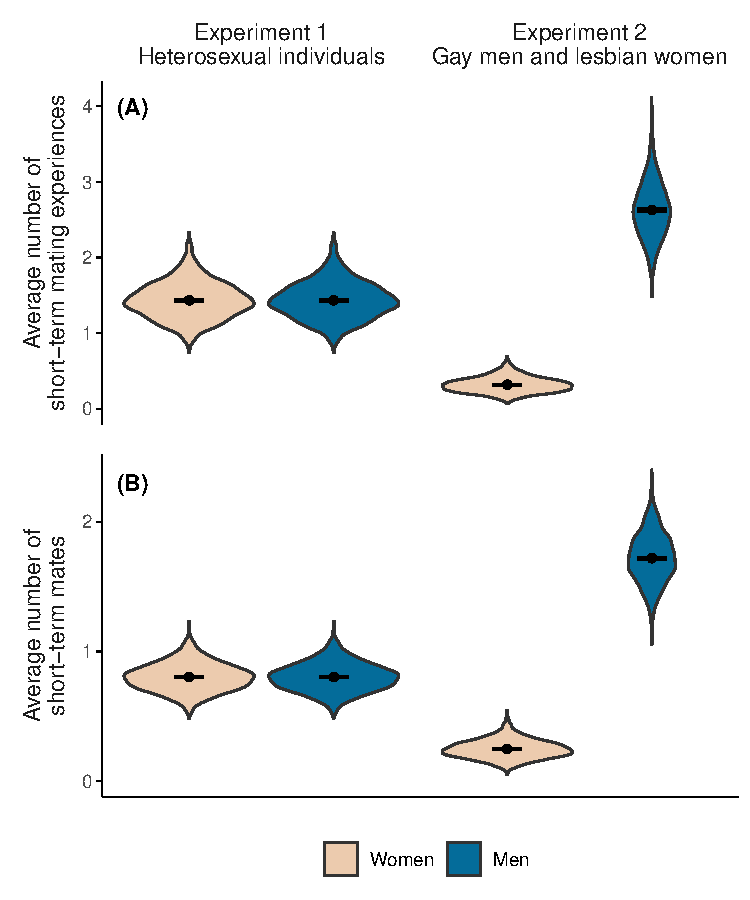
\includegraphics[width=80mm]{figures/fig1_men_vs_women.pdf}
  \caption{\textbf{Short-term mating behaviors of men and women after 1,000 time steps in the model when gender differences existed in mating preferences.} Violin plots summarizing the outcome variables separately for heterosexual individuals and gay men and lesbian women. Plot (A) shows the average number of short-term mating experiences, and plot (B) shows the average number of short-term mates. Central points show mean values and whiskers represent standard errors, but the standard errors are small and overlap to form a single bar. Statistics were calculated using the full population of men and women in the model (\textit{N\textsubscript{m}} = \textit{N\textsubscript{w}} = 150).}
\end{figure}

The results from Experiment 2 showed that when there were gender
differences in preferences for short-term mating, there were gender
differences in short-term mating behaviors between gay men and lesbian
women (Figure 1). The average number of short-term mating experiences
was higher among gay men (\emph{M} = 2.63, \emph{SD} = 0.37) than among
lesbian women (\emph{M} = 0.32, \emph{SD} = 0.10), \emph{t}(4,998) =
-301.78, \emph{p} \textless{} .001, Cohen's \emph{d} = 8.54. Similarly,
the average number of short-term mates was higher among gay men
(\emph{M} = 1.72, \emph{SD} = 0.19) than among lesbian women (\emph{M} =
0.25, \emph{SD} = 0.07), \emph{t}(4,998) = -357.69, \emph{p} \textless{}
.001, Cohen's \emph{d} = 10.12.

In Experiment 1, however, when the means of the outcome variables were
calculated among men and women who were in the mating pool (i.e., those
with a non-zero number of short-term mating experiences) \textbf{(the
number of individuals in the mating pool: M\textsubscript{m},
SD\textsubscript{m}; M\textsubscript{w}, SD\textsubscript{w})}, there
were gender differences in short-term mating behaviors when there were
gender differences in mating preferences. The average number of
short-term mating experiences was higher among heterosexual men
(\emph{M} = 3.78, \emph{SD} = 0.50) than among heterosexual women
(\emph{M} = 2.79, \emph{SD} = 0.35), \emph{t}(4,998) = -81.53, \emph{p}
\textless{} .001, Cohen's \emph{d} = 2.31. Likewise, the average number
of short-term mates was higher among heterosexual men (\emph{M} = 2.12,
\emph{SD} = 0.17) than among heterosexual women (\emph{M} = 1.56,
\emph{SD} = 0.11), \emph{t}(4,998) = -135.85, \emph{p} \textless{} .001,
Cohen's \emph{d} = 3.84.

\hypertarget{comparing-short-term-mating-behaviors-of-heterosexual-and-gay-men}{%
\subsection{Comparing short-term mating behaviors of heterosexual and
gay
men}\label{comparing-short-term-mating-behaviors-of-heterosexual-and-gay-men}}

The results comparing across the two experiments revealed that gay men
engaged in short-term mating behaviors more than heterosexual men did
(Figure 2). The average number of short-term mating experiences was
higher among gay men (\emph{M} = 2.63, \emph{SD} = 0.37) than among
heterosexual men (\emph{M} = 1.43, \emph{SD} = 0.24), \emph{t}(4,998) =
-134.87, \emph{p} \textless{} .001, Cohen's \emph{d} = 3.81. Similarly,
the average number of short-term mates was higher among gay men
(\emph{M} = 1.72, \emph{SD} = 0.19) than among heterosexual men
(\emph{M} = 0.80, \emph{SD} = 0.11), \emph{t}(4,998) = -206.91, \emph{p}
\textless{} .001, Cohen's \emph{d} = 5.85.

\begin{figure}[h]
  \centering
  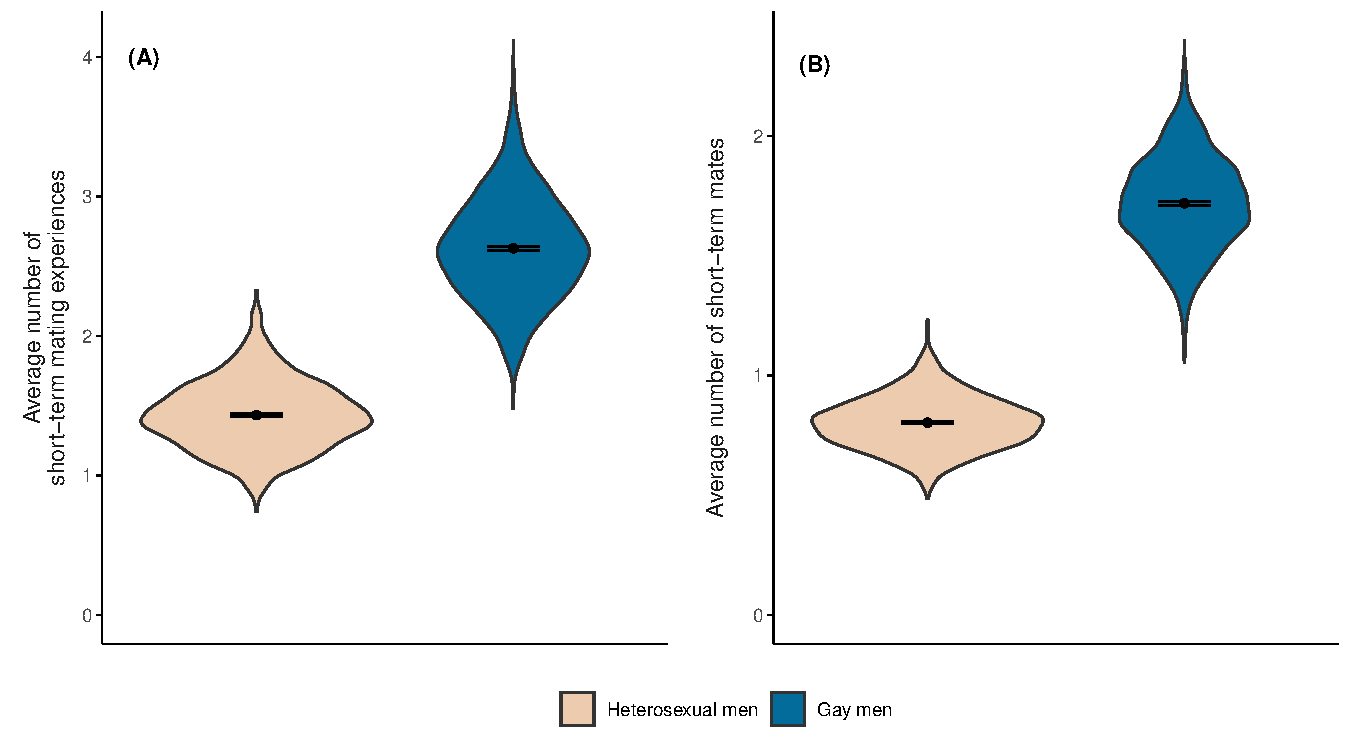
\includegraphics[width=0.8\columnwidth]{figures/fig2_hetero_vs_gay_men.pdf}
  \caption{\textbf{Short-term mating behaviors of heterosexual and gay men after 1,000 time steps in the model when gender differences existed in mating preferences.} Violin plots summarizing the outcome variables. Plot (A) shows the average number of short-term mating experiences, and plot (B) shows the average number of short-term mates. Central points show mean values and whiskers represent standard errors, but the standard errors are small and overlap to form a single bar. Statistics were calculated using the full population of heterosexual and gay men in the model (\textit{N\textsubscript{hm}} = \textit{N\textsubscript{gm}} = 150).}
\end{figure}

\hypertarget{comparing-across-conditions}{%
\subsection{Comparing across
conditions}\label{comparing-across-conditions}}

In an exploratory manner, we also compared across conditions to see
which of the two dimensions of preferences for short-term mating
contributed to gender differences in sexual behaviors.

Among heterosexual individuals, gender differences in short-term mating
behaviors, as calculated among individuals in the mating pool, emerged
when men and women had different standards for short-term mates.
Heterosexual men in the mating pool had a higher average number of
short-term mating experiences and short-term mates than women in the
mating pool, even when no gender difference existed in short-term mating
likelihood (experiences: \emph{M\textsubscript{m}} = 2.82,
\emph{SD\textsubscript{m}} = 0.36, \emph{M\textsubscript{w}} = 2.21,
\emph{SD\textsubscript{w}} = 0.28, Cohen's \emph{d} = 1.89; partners:
\emph{M\textsubscript{m}} = 1.76, \emph{SD\textsubscript{m}} = 0.15;
\emph{M\textsubscript{w}} = 1.38, \emph{SD\textsubscript{w}} = 0.09,
Cohen's \emph{d} = 3.13). In comparison, virtually no gender differences
in short-term mating behaviors existed when men and women had the same
mating standards (Table 1).

\begin{table}

\caption{\label{tab:table_1}\textbf{Short-term mating behaviors of heterosexual men and women in the mating pool after 1,000 time steps in the model}}
\centering
\begin{threeparttable}
\resizebox{\linewidth}{!}{
\begin{tabular}[t]{>{\raggedright\arraybackslash}p{2in}llllllllll}
\toprule
\multicolumn{1}{c}{ } & \multicolumn{5}{c}{\makecell[c]{Average short-term mating\\experiences (in-pool)}} & \multicolumn{5}{c}{\makecell[c]{Average short-term\\mates (in-pool)}} \\
\cmidrule(l{3pt}r{3pt}){2-6} \cmidrule(l{3pt}r{3pt}){7-11}
\multicolumn{1}{c}{ } & \multicolumn{2}{c}{Men} & \multicolumn{2}{c}{Women} & \multicolumn{1}{c}{ } & \multicolumn{2}{c}{Men} & \multicolumn{2}{c}{Women} & \multicolumn{1}{c}{ } \\
\cmidrule(l{3pt}r{3pt}){2-3} \cmidrule(l{3pt}r{3pt}){4-5} \cmidrule(l{3pt}r{3pt}){7-8} \cmidrule(l{3pt}r{3pt}){9-10}
\multicolumn{1}{c}{\em{ }} & \multicolumn{1}{c}{\em{M}} & \multicolumn{1}{c}{\em{SD}} & \multicolumn{1}{c}{\em{M}} & \multicolumn{1}{c}{\em{SD}} & \multicolumn{1}{c}{\em{d}} & \multicolumn{1}{c}{\em{M}} & \multicolumn{1}{c}{\em{SD}} & \multicolumn{1}{c}{\em{M}} & \multicolumn{1}{c}{\em{SD}} & \multicolumn{1}{c}{\em{d}}\\
\midrule
Same likelihood*Same standard & 2.21 & 0.38 & 2.20 & 0.37 & 0.03 & 1.39 & 0.12 & 1.39 & 0.12 & 0.04\\
Same likelihood*Different standard & 2.82 & 0.36 & 2.21 & 0.28 & 1.89 & 1.76 & 0.15 & 1.38 & 0.09 & 3.13\\
Different likelihood*Same standard & 2.80 & 0.48 & 2.78 & 0.47 & 0.03 & 1.57 & 0.14 & 1.56 & 0.14 & 0.05\\
Different likelihood*Different standard & 3.78 & 0.50 & 2.79 & 0.35 & 2.31 & 2.12 & 0.17 & 1.56 & 0.11 & 3.84\\
\bottomrule
\end{tabular}}
\begin{tablenotes}
\small
\item \textit{Note.} The statistics were calculated with subsamples of men and women who had had enagged in short-term mating behaviors. See Supplementary Materials for the mean and standard deviation of sample sizes.
\end{tablenotes}
\end{threeparttable}
\end{table}

Among gay men and lesbian women, gender differences in short-term mating
behaviors emerged either when they had different short-term mating
likelihood or when their mating standards were different. Gay men had a
higher average number of short-term mating experiences and short-term
mates when they had a higher short-term mating likelihood than lesbian
women (experiences: \emph{M\textsubscript{m}} = 0.80,
\emph{SD\textsubscript{m}} = 0.23, \emph{M\textsubscript{w}} = 0.32,
\emph{SD\textsubscript{w}} = 0.10, Cohen's \emph{d} = 2.67; partners:
\emph{M\textsubscript{m}} = 0.52, \emph{SD\textsubscript{m}} = 0.13,
\emph{M\textsubscript{w}} = 0.25, \emph{SD\textsubscript{w}} = 0.07,
Cohen's \emph{d} = 2.60), or when they had a lower mating standards
(experiences: \emph{M\textsubscript{m}} = 1.05,
\emph{SD\textsubscript{m}} = 0.18, \emph{M\textsubscript{w}} = 0.32,
\emph{SD\textsubscript{w}} = 0.10, Cohen's \emph{d} = 5.10; partners:
\emph{M\textsubscript{m}} = 0.82, \emph{SD\textsubscript{m}} = 0.12,
\emph{M\textsubscript{w}} = 0.25, \emph{SD\textsubscript{w}} = 0.07,
Cohen's \emph{d} = 5.78). In comparison, virtually no gender differences
in short-term mating behaviors existed when gay men and lesbian women
had the same short-term mating likelihood and mating standards (Table
2).

\begin{table}

\caption{\label{tab:table_2}\textbf{Short-term mating behaviors of gay men and lesbian women after 1,000 time steps in the model}}
\centering
\begin{threeparttable}
\resizebox{\linewidth}{!}{
\begin{tabular}[t]{>{\raggedright\arraybackslash}p{2in}llllllllll}
\toprule
\multicolumn{1}{c}{ } & \multicolumn{5}{c}{\makecell[c]{Average short-term mating\\experiences}} & \multicolumn{5}{c}{Average short-term mates} \\
\cmidrule(l{3pt}r{3pt}){2-6} \cmidrule(l{3pt}r{3pt}){7-11}
\multicolumn{1}{c}{ } & \multicolumn{2}{c}{Men} & \multicolumn{2}{c}{Women} & \multicolumn{1}{c}{ } & \multicolumn{2}{c}{Men} & \multicolumn{2}{c}{Women} & \multicolumn{1}{c}{ } \\
\cmidrule(l{3pt}r{3pt}){2-3} \cmidrule(l{3pt}r{3pt}){4-5} \cmidrule(l{3pt}r{3pt}){7-8} \cmidrule(l{3pt}r{3pt}){9-10}
\multicolumn{1}{c}{\em{ }} & \multicolumn{1}{c}{\em{M}} & \multicolumn{1}{c}{\em{SD}} & \multicolumn{1}{c}{\em{M}} & \multicolumn{1}{c}{\em{SD}} & \multicolumn{1}{c}{\em{d}} & \multicolumn{1}{c}{\em{M}} & \multicolumn{1}{c}{\em{SD}} & \multicolumn{1}{c}{\em{M}} & \multicolumn{1}{c}{\em{SD}} & \multicolumn{1}{c}{\em{d}}\\
\midrule
Same likelihood*Same standard & 0.32 & 0.10 & 0.32 & 0.10 & 0.04 & 0.25 & 0.07 & 0.25 & 0.07 & 0.03\\
Same likelihood*Different standard & 1.05 & 0.18 & 0.32 & 0.10 & 5.10 & 0.82 & 0.12 & 0.25 & 0.07 & 5.78\\
Different likelihood*Same standard & 0.80 & 0.23 & 0.32 & 0.10 & 2.67 & 0.52 & 0.13 & 0.25 & 0.07 & 2.60\\
Different likelihood*Different standard & 2.63 & 0.37 & 0.32 & 0.10 & 8.54 & 1.72 & 0.19 & 0.25 & 0.07 & 10.12\\
\bottomrule
\end{tabular}}
\begin{tablenotes}
\small
\item \textit{Note.} \textit{N\textsubscript{m}} = \textit{N\textsubscript{w}} = 150 in all conditions.
\end{tablenotes}
\end{threeparttable}
\end{table}

\hypertarget{discussion}{%
\section{Discussion}\label{discussion}}

The present study aimed at using agent-based modeling to investigate
whether men and women's different mating preferences resulted in any
gender differences in short-term mating behaviors, specifically, in the
number of short-term mating experiences and short-term mates, and if
they did, under what circumstances. We raised two hypotheses: 1) there
would be gender differences in short-term mating behaviors among gay men
and lesbian women, with gay men being engaged in more such behaviors,
and 2) gay men would engage in more short-term mating behaviors as
compared to heterosexual men. The results from 1,000 time steps in a
model simulating men and women's mating behaviors supported our
hypotheses. First of all, as compared to lesbian women, gay men had a
higher average number of short-term mating experiences and short-term
mates. In contrast, we found no gender differences in short-term mating
behaviors between heterosexual men and women. Secondly, gay men also had
a higher average number of short-term mating experiences and short-term
mates as compared to heterosexual men.

As we expected, heterosexual men and women did not differ in short-term
mating behaviors despite their different mating preferences. This was
because the total numbers of short-term mating experiences and
short-term mates of heterosexual men and women were exactly the same.
Since the sex ratio was 1:1 in our model, the average number of
short-term mating experiences and short-term mates must be equal between
men and women as well. However, we did find that among individuals in
the mating pool, men engaged in more short-term mating behaviors as
compared to women. This was because there were more women than men in
the mating pool (i.e., had ever engaged in short-term mating behaviors),
resulting in lower averages among heterosexual women despite equal
numbers of experiences and mates in total.

Moreover, gender differences in short-term mating behaviors emerged when
heterosexual men and women had different standards for short-term mates,
but not when they had different likelihood of engaging in short-term
mating. When women had a higher standard than men did, less men than
women in the population were above a potential partner's standards and
thus had a chance to have sex with them. This contributed to the unequal
number of men and women in the mating pool, which led to gender
differences in short-term mating behaviors.

In the light of these results, the empirical observation of gender
differences in short-term mating behaviors among heterosexual
individuals (e.g., Petersen \& Hyde, 2010) appear to be perplexing
because this is theoretically illogical (e.g., Gurman, 1989). Possible
explanations for these empirical results have to highlight caveats in
the observation process. One possibility is that there was sampling bias
in the observations (e.g., Wiederman \& Dubois, 1998) since surveys
regarding short-term mating behaviors may tend to attract individuals
who already engage in such behaviors. Another possibility is that
heterosexual men and women tend to report short-term mating behaviors
differently. This difference may be a result of social desirability bias
(Alexander \& Fisher, 2003) or due to men and women's different
estimation strategies (e.g., men tend to round up) (Brown \& Sinclair,
1999).

Among gay men and lesbian women, large gender differences in short-term
mating behaviors existed when men and women had different mating
preferences, which was in line with empirical observations (e.g., Peplau
et al., 1997, 2004). This was probably because the number of short-term
mating experiences and short-term mates no longer counted towards men
and women simultaneously. Any gender differences in mating preferences
would result in differences in behaviors. A closer look at the results
did support this postulation. Either a difference in the likelihood of
short-term mating or a difference in mating standards alone could
contribute to gender differences in mating behaviors. This was perhaps
because the former increased the probability of both parties of a given
gay couple deciding to have short-term mating, and the latter increased
the probability of both of them meeting each other's standards, as
compared to the case of a given lesbian couple.

Supporting the idea that gay men's preferences for short-term mating
were not constrained by those of women, we found that gay men engaged in
more short-term mating behaviors as compared to heterosexual men. This
was consistent with the empirical literature (e.g., Peplau et al.,
1997). Interestingly, gay men and heterosexual men had the same
likelihood of short-term mating and the same standards for short-term
mates in our model. The only difference was a change in the preferences
in their potential partners. When men's partners had a stronger
preferences for short-term mating (i.e., having men vs.~having women as
potential partners), men also appeared to engage in more short-term
mating behaviors.

\hypertarget{conclusion}{%
\section{Conclusion}\label{conclusion}}

Using agent-based modeling, the present study theoretically explored the
circumstances under which men and women's different mating preferences
resulted in gender differences in short-term mating behaviors. We found
when men (vs.~women) had a stronger preferences for short-term mating,
heterosexual men and women engaged in short-term mating behaviors to the
same extent, while gay men engaged in more short-term mating behaviors
as compared to lesbian women. We also found that gay men engaged in more
short-term mating behaviors than heterosexual men did.

Theses results highlight the distinction between psychological
preferences and behaviors in human mating. Individuals' mating behaviors
do not only depend on one's own preferences, but are also constrained by
partners' preferences. Future research in human mating should not only
focus on the psychological aspect but also pay attention to the
interaction between individuals' psychology and its context. These
results also cast doubt to the prevalent belief in the gender
differences in short-term mating behaviors, especially among
heterosexual individuals. Our findings suggest that there may be factors
in the observation process that lead to such differences. Future
research in human sexuality should note such possibilities and interpret
any observed gender differences in short-term mating behaviors
cautiously.

\hypertarget{acknowledgements}{%
\section{Acknowledgements}\label{acknowledgements}}

\hypertarget{data-availability}{%
\section{Data availability}\label{data-availability}}

All models, data, and analysis code can be downloaded at: {[}link masked
for peer review{]}

\newpage

\hypertarget{references}{%
\section*{References}\label{references}}
\addcontentsline{toc}{section}{References}

\hypertarget{refs}{}
\begin{CSLReferences}{1}{0}
\leavevmode\vadjust pre{\hypertarget{ref-alexander_truth_2003}{}}%
Alexander, M. G., \& Fisher, T. D. (2003). Truth and consequences: Using
the bogus pipeline to examine sex differences in self‐reported
sexuality. \emph{The Journal of Sex Research}, \emph{40}(1), 27--35.
\url{https://doi.org/10.1080/00224490309552164}

\leavevmode\vadjust pre{\hypertarget{ref-archer_reality_2019}{}}%
Archer, J. (2019). The reality and evolutionary significance of human
psychological sex differences. \emph{Biological Reviews}, \emph{94}(4),
1381--1415. \url{https://doi.org/10.1111/brv.12507}

\leavevmode\vadjust pre{\hypertarget{ref-bailey_effects_1994}{}}%
Bailey, J. M., Gaulin, S., Agyei, Y., \& Gladue, B. A. (1994). Effects
of gender and sexual orientation on evolutionarily relevant aspects of
human mating psychology. \emph{Journal of Personality and Social
Psychology}, \emph{66}(6), 1081--1093.
\url{https://doi.org/10.1037/0022-3514.66.6.1081}

\leavevmode\vadjust pre{\hypertarget{ref-brown_estimating_1999}{}}%
Brown, N. R., \& Sinclair, R. C. (1999). Estimating number of lifetime
sexual partners: Men and women do it differently. \emph{The Journal of
Sex Research}, \emph{36}(3), 292--297.
\url{https://doi.org/10.1080/00224499909551999}

\leavevmode\vadjust pre{\hypertarget{ref-bryant_relationship_1994}{}}%
Bryant, A. S., \& Demian. (1994). Relationship characteristics of
american gay and lesbian couples. \emph{Journal of Gay \& Lesbian Social
Services}, \emph{1}(2), 101--117.
\url{https://doi.org/10.1300/J041v01n02_06}

\leavevmode\vadjust pre{\hypertarget{ref-buss_sexual_1993}{}}%
Buss, D. M., \& Schmitt, D. P. (1993). Sexual strategies theory: An
evolutionary perspective on human mating. \emph{Psychological Review},
\emph{100}(2), 204--232.
\url{https://doi.org/doi:10.1037/0033-295X.100.2.204d}

\leavevmode\vadjust pre{\hypertarget{ref-conley_women_2011}{}}%
Conley, T. D., Moors, A. C., Matsick, J. L., Ziegler, A., \& Valentine,
B. A. (2011). Women, men, and the bedroom: Methodological and conceptual
insights that narrow, reframe, and eliminate gender differences in
sexuality. \emph{Current Directions in Psychological Science},
\emph{20}(5), 296--300. \url{https://doi.org/10.1177/0963721411418467}

\leavevmode\vadjust pre{\hypertarget{ref-s_j_gurman_six_1989}{}}%
Gurman, S. J. (1989). Six of one... \emph{Nature}, \emph{12}, 342.
\url{https://www.nature.com/articles/342012d0}

\leavevmode\vadjust pre{\hypertarget{ref-hald_receptivity_2010}{}}%
Hald, G. M., \& Høgh-Olesen, H. (2010). Receptivity to sexual
invitations from strangers of the opposite gender. \emph{Evolution and
Human Behavior}, \emph{31}(6), 453--458.
\url{https://doi.org/10.1016/j.evolhumbehav.2010.07.004}

\leavevmode\vadjust pre{\hypertarget{ref-herbenick_sexual_2017}{}}%
Herbenick, D., Bowling, J., Fu, T.-C. (Jane)., Dodge, B., Guerra-Reyes,
L., \& Sanders, S. (2017). Sexual diversity in the {United States}:
Results from a nationally representative probability sample of adult
women and men. \emph{{PLOS} {ONE}}, \emph{12}(7), e0181198.
\url{https://doi.org/10.1371/journal.pone.0181198}

\leavevmode\vadjust pre{\hypertarget{ref-kenrick_evolution_1990}{}}%
Kenrick, D. T., Sadalla, E. K., Groth, G., \& Trost, M. R. (1990).
Evolution, traits, and the stages of human courtship: Qualifying the
parental investment model. \emph{Journal of Personality}, \emph{58}(1),
97--116. \url{https://doi.org/10.1111/j.1467-6494.1990.tb00909.x}

\leavevmode\vadjust pre{\hypertarget{ref-matsick_gender_2021}{}}%
Matsick, J. L., Kruk, M., Conley, T. D., Moors, A. C., \& Ziegler, A.
(2021). Gender similarities and differences in casual sex acceptance
among lesbian women and gay men. \emph{Archives of Sexual Behavior},
\emph{50}(3), 1151--1166.
\url{https://doi.org/10.1007/s10508-020-01864-y}

\leavevmode\vadjust pre{\hypertarget{ref-mcburney_preferred_2005}{}}%
McBurney, D. H., Zapp, D. J., \& Streeter, S. A. (2005). Preferred
number of sexual partners: Tails of distributions and tales of mating
systems. \emph{Evolution and Human Behavior}, \emph{26}(3), 271--278.
\url{https://doi.org/10.1016/j.evolhumbehav.2004.09.005}

\leavevmode\vadjust pre{\hypertarget{ref-oliver_gender_1993}{}}%
Oliver, M. B., \& Hyde, J. S. (1993). Gender differences in sexuality: A
meta-analysis. \emph{Psychological Bulletin}, \emph{114}(1), 29--51.
https://doi.org/\url{http://dx.doi.org/10.1037/0033-2909.114.1.29}

\leavevmode\vadjust pre{\hypertarget{ref-peplau_national_1997}{}}%
Peplau, L. A., Cochran, S. D., \& Mays, V. (1997). A national survey of
the intimate relationships of african american lesbians and gay men: A
look at commitment, satisfaction, sexual behavior, and {HIV} disease. In
\emph{Ethnic and cultural diversity among lesbians and gay men} (pp.
11--38). Sage Publications.

\leavevmode\vadjust pre{\hypertarget{ref-peplau_sexuality_2004}{}}%
Peplau, L. A., Fingerhut, A., \& Beals, K. P. (2004). Sexuality in the
relationships of lesbians and gay men. In \emph{The handbook of
sexuality in close relationships} (pp. 349--369). Lawrence Erlbaum
Associates Publishers.

\leavevmode\vadjust pre{\hypertarget{ref-petersen_meta-analytic_2010}{}}%
Petersen, J. L., \& Hyde, J. S. (2010). A meta-analytic review of
research on gender differences in sexuality, 1993--2007.
\emph{Psychological Bulletin}, \emph{136}(1), 21--38.
\url{https://doi.org/10.1037/a0017504}

\leavevmode\vadjust pre{\hypertarget{ref-r}{}}%
R Core Team. (2022). \emph{R: A language and environment for statistical
computing}. R Foundation for Statistical Computing.
\url{https://www.R-project.org/}

\leavevmode\vadjust pre{\hypertarget{ref-regan_minimum_1998}{}}%
Regan, P. C. (1998). Minimum mate selection standards as a function of
perceived mate value, relationship context, and gender. \emph{Journal of
Psychology \& Human Sexuality}, \emph{10}(1), 53--73.
\url{https://doi.org/10.1300/J056v10n01_04}

\leavevmode\vadjust pre{\hypertarget{ref-rissel_heterosexual_2014}{}}%
Rissel, C., Badcock, P. B., Smith, A. M. A., Richters, J., Visser, R. O.
de, Grulich, A. E., Simpson, J. M., Rissel, C., Badcock, P. B., Smith,
A. M. A., Richters, J., Visser, R. O. de, Grulich, A. E., \& Simpson, J.
M. (2014). Heterosexual experience and recent heterosexual encounters
among {A}ustralian adults: The second {A}ustralian study of health and
relationships. \emph{Sexual Health}, \emph{11}(5), 416--426.
\url{https://doi.org/10.1071/SH14105}

\leavevmode\vadjust pre{\hypertarget{ref-schmitt_universal_2003}{}}%
Schmitt, D. P. (2003). Universal sex differences in the desire for
sexual variety: Tests from 52 nations, 6 continents, and 13 islands.
\emph{Journal of Personality and Social Psychology}, \emph{85}(1), 85.
\url{https://doi.org/10.1037/0022-3514.85.1.85}

\leavevmode\vadjust pre{\hypertarget{ref-schmitt_are_2001}{}}%
Schmitt, D. P., Shackelford, T. K., \& Buss, D. M. (2001). Are men
really more 'oriented' toward short-term mating than women? A critical
review of theory and research. \emph{Psychology, Evolution \& Gender},
\emph{3}(3), 211--239. \url{https://doi.org/10.1080/14616660110119331}

\leavevmode\vadjust pre{\hypertarget{ref-symons_evolution_1979}{}}%
Symons, D. (1979). \emph{The evolution of human sexuality}. Oxford
University Press.

\leavevmode\vadjust pre{\hypertarget{ref-walter_sex_2020}{}}%
Walter, K. V., Conroy-Beam, D., Buss, D. M., Asao, K., Sorokowska, A.,
Sorokowski, P., Aavik, T., Akello, G., Alhabahba, M. M., Alm, C., Amjad,
N., Anjum, A., Atama, C. S., Atamtürk Duyar, D., Ayebare, R., Batres,
C., Bendixen, M., Bensafia, A., Bizumic, B., \ldots{} Zupančič, M.
(2020). Sex differences in mate preferences across 45 countries: A
large-scale replication. \emph{Psychological Science}, \emph{31}(4),
408--423. \url{https://doi.org/10.1177/0956797620904154}

\leavevmode\vadjust pre{\hypertarget{ref-ggplot2}{}}%
Wickham, H. (2016). \emph{{ggplot2: Elegant Graphics for Data
Analysis}}. Springer-Verlag New York.
\url{https://ggplot2.tidyverse.org}

\leavevmode\vadjust pre{\hypertarget{ref-wiederman_evolution_1998}{}}%
Wiederman, M. W., \& Dubois, S. L. (1998). Evolution and sex differences
in preferences for short-term mates: Results from a policy capturing
study. \emph{Evolution and Human Behavior}, \emph{19}(3), 153--170.
\url{https://doi.org/10.1016/S1090-5138(98)00006-3}

\leavevmode\vadjust pre{\hypertarget{ref-wilensky_1999}{}}%
Wilensky, U. (1999). \emph{NetLogo}
{[}Http://ccl.northwestern.edu/netlogo/{]}. Center for Connected
Learning; Computer-Based Modeling.
\url{http://ccl.northwestern.edu/netlogo/}

\end{CSLReferences}

\end{document}
